\chapter{Multi-Cloud-Anwendungs-Broker}
\label{cha:broker}

% Vorteile
% Neue Märkte in anderen Regionen der Welt
% Schnelles Ausrollen neuer Apps
% DevOps geeignet
% Risikoreduzierung
% Reduzierung von (gleichzeitig) Investitionsausgaben und Betriebskosten
% Bestehende Cloud-Deployments mit verwalten-

Um eine Anwendung automatisiert auf verschiedene Clouds zu verteilen ist ein Broker-Mechanismus nötig. Dieser sollte nach verschiedenen, festzulegenden Kriterien vorgehen. Konkret erfüllt ein Broker in der Regel folgende Aufgaben:

\begin{enumerate}
	\item Bereitstellen der Ressourcen für eine Applikation; starten einer virtuellen Maschine oder Reservierung von Speicherplatz
	\item Starten der Anwendung auf den vorher reservierten Ressourcen
	\item Verteilen eingehender Anfragen auf gestartete Anwendungs-Instanzen
	\item Management der Ressourcen
\end{enumerate}

\noindent
Zusätzlich sollte der Multi-Cloud-Broker Policys und SLAs auswerten und umsetzen können. Denkbar ist das automatische Re-provisionieren anhand von 

\begin{enumerate}
	\item Lastspitzen oder Ausfällen von Hardware und Netzwerkressourcen 
	%	(Monitoring)
	\item Geänderten Umfeldparametern wie der Gesetzgebung, Preisen oder AGBs
	\item Nutzeränderungen
	\item Vorherigen Broker-Aktionen
\end{enumerate}

\noindent
In einer Community Cloud könnten Cloud-Provider selbst einen Mechanismus zum Brokering oder zumindest offene APIs bereitstellen. Der Broker wäre also Teil der Cloud. Möglich sind entweder ein zentraler Broker, der direkt auf Cloud-Interna zugreift, oder aber ein Peer-to-Peer-Verbund.\todo{Grafik Architekturübersicht}

Für Multi-Clouds kommen diese Lösungen nicht infrage: Sie bestehen aus mehreren unabhängigen, meist privaten, Cloud-Providern. Aufgrund gegenläufiger Geschäftsinteressen sind diese nicht an einer Föderation mit anderen Anbietern interessiert. Sie werden also weder Interna ihrer Cloud-Plattform anpassen, noch einheitliche APIs bereitstellen.

Stattdessen muss der Broker in einer Multi-Cloud-Umgebung extern bereitgestellt werden. In diesem Fall kann er entweder als eigenständiger Service in Form einer \emph{Cloud Management Platform} angelegt sein, oder von der verteilten Anwendung selbst implementiert werden. Selbst entwickelte CMPs oder integrierte Broker setzen oft auf Multi-Cloud-Bibliotheken wie \emph{Apache libcloud}. \autoref{sec:bibliotheken} bietet hierzu eine Übersicht aktueller Open Source-Projekte. 

Folgende weitere Aspekte sollen bei der Betrachtung der CMPs berücksichtigt werden:

\begin{description}
	
	\item[Zielgruppe] 	\emph{Entwickler und Administratoren}: Im Rahmen von DevOps stellen sie verschiedene Ausführungsumgebungen für Entwicklung, Test und Produktion bereit. Dabei nutzen sie die Self-Service-Funktionen der CMPs.
	
						\emph{Management}: Die Auslastungs- und Kostenübersicht ermöglicht weitere Planung. SLAs und Policys werden überwacht und durchgesetzt.
	
	\item[Anwendungen] Grundsätzlich alle interaktiven Anwendungen und Dienste, sowie Stapelverarbeitungs-Jobs. Diese können verteilt sein. Die CMP muss in diesem Fall z.\,B. die Nähe des Datenspeichers zur Rechen-Einheiten beachten.
	
	Ausgenommen: spezielle Big Data Analytics und Forschungsszenarien, die unter Umständen besondere Features, Rechte und Architekturen benötigen.
	
	\item[Funktionsumfang] Über die grundlegende Provisionierung hinaus sollte die CMP auch bei weiteren Orchestrationsaufgaben unterstützen: Konfiguration, Monitoring und Skalierung.
%	https://dzone.com/articles/cloud-management-roundup-orchestration-vs-paas-vs-cmp
	
	Die Unterstützung aktueller Container-Technologien und Cloud-Native-Architekturen ist wünschenswert. Keine Rolle spielt \emph{Bare Metal}: Eine installierte Virtualisierungsschicht oder Container-Laufzeitumgebung wird vorausgesetzt. 
	
	Die Auswertung der SLAs und Policys ist auf die verteilten Anwendungen selbst beschränkt. Darüber liegende (CMP-Nutzer) oder tiefergehende Schichten (Service-Nutzer und -Daten) werden extern verwaltet.
		
\end{description}


\noindent
Der folgende Abschnitt gibt eine Übersicht kommerzieller Cloud Management Plattformen sowie bisheriger Forschung zu Inter- und Multi-Cloud-Brokern mit besonderem Blick auf SLAs und Policys. Die vorgestellten Lösungen unterscheiden sich in Architektur, Flexibilität und Funktionsumfang. Die vier anfangs vorgestellten Broker-Basiseigenschaften werden nicht von allen Arbeiten in vollem Umfang erfüllt.

Weiterhin zeigen wir einheitliche Ansätze zu maschinenlesbaren Policy- und SLA-Definitionen. Anschließend entwickeln wir ein Service-Schema für den Multi-Cloud-Einsatz. Es folgen der Vorschlag für ein Broker-Design und passende Matching-Algorithmen.



\section{Maschinenlesbare SLA- und Policy-Schemata}

Templates und Agreements. Hier eher Templates.

Kontext: Provider, Kunde, Gültigkeitszeitraum usw.
Stattdessen Abbildung der SLOs.

Service-Level statt Customer-level oder mUlti-Level:.

Broker, nicht Mediator. Also keine Verhandlung.

1. Lesen der Provider-Angebote in einem einheitlichen Format (unmöglich)
   Für private Clouds manuell feststellbar
2. Definition von Anforderungen auf Anwendungs-Ebene
3. Abgleich der Angebote und Deployment
4. Überwachung auf Einhaltung
5. Reaktion: Re-deployment und Schadensersatz (muss automatisch abgewickelt werden, die Erleichterung durch Cloud fällt sonst deutlich kleiner aus)

Das Monitoring tool muss slas verstehen

 
Implementiert?
Auch für Menschen verständlich?
Vorstellungs-Paper!

Übersicht: 
%Service Level Agreement Mediation,
%Negotiation and Evaluation for
%Cloud Services in Intercloud Environments
%vorgelegt von
%M.Sc. Dipl.-Ing. (FH)
%Alexander Stanik
% Externer Mediator zwischen Provider und Kunden. Im Gegensatz hierzu wollen wir SLAs nicht verhandeln. Public Cloud Provider bieten Kleinkunden keine individuellen Angebote. Dies nehmen wir als gegeben. Stattdessen sucht der Broker anhand bestimmter Anforderungen eine passende Kombination aus einem oder mehreren Cloud-Angeboten.
%=> Kein Verhandlungsframework.

ganzes Framework oder SLA-Schema?
Erstellen, Anbieten, Verhandeln, Überwachen

\begin{description}
	\item[Web Services Agreement Specification (WS-Agreement)]
	Open Grid Forum (OGF), unter anderem IBM,  2007
	XML
	Web Services SOAP
	
	Teil der WS-* Spezifikationen
	
	Aushandeln nur per Erweiterung \emph{WS-Agreement Negotiation}
	
	Oberflächlicher, generischer, keine Sprachelemente zur Beschreibung von Metriken, logischen Operatoren und Prädikaten.
	
	Keine komplexen Metriken oder Prädikaten ohne Erweiterung, kleinerer Sprachumfang. Leichter Einstieg, Fokus: SLA-Lebenszyklus
	
	für jedes praxisrelevante SLA domänenspezifische Erweiterungen mit entsprechenden Metriken.

	
%	A. Andrieux, K. Czajkowski, A. Dan, et al, Web Services
%	Agreement Specification (WS-Agreement), March 14 2007,
%	available at: http://www.ogf.org/documents/GFD.107.pdf
	
	Implementierungen?	
	%	http://wsag4j.sourceforge.net/site/wsag/wsag-language.html
%	https://link.springer.com/chapter/10.1007/978-3-319-11746-1_21
	RESTful statt SOAP
	
	\item[Web Service Level Agreement (WSLA)] wurde 2003 von IBM vorgestellt und basiert ebenso auf XML. 
	
	Details, egnaue Beschreibung was wie oft zu messen ist, sowie die Aktion bei EIntreffen
	
	Einbinden von Referenzen auf WSDL (zur Modellierung von Services selbst).
	
	Funktionen, Erweiterbar, zusammengesetzte Metriken, und Vererbung.
	
	Fokus: Metriken
	
	Beide Vertragspartner, WSLA modelliert Angebot und Anforderungen gleichermaßen. Überwachung und Auswertung können von einer dritten Partei implementiert werden.
	
		
%H. Ludwig, A. Keller, A. Dan, et al, Web Service
%Level Agreement (WSLA) Language Specification, January
%28 2003, available at: http://www.research.ibm.com/wsla/
%WSLASpecV1-20030128.pdf

=> Beide nutzen XML. Besonderheit: Direkt mit ITIL und dessen Vertragsobjekten nutzbar.
%	Köhler, Peter T.: ITIL: Das IT-Servicemanagement Framework. 2007
 Zwar streng formalisiert und durch verfügbare Schemata gut zu verarbeiten, für Menschen aber nur schwer les- und editierbar.


%	\item[SMI (STRATOS)] 




	\item[OCCI SLAs]


%	https://github.com/IntelLabsEurope/OCCI-SLAs



	\item[TOSCA Policys] asdasd
	
	asdasdasd
	
	\begin{listing}[ht]
		\inputminted[]{yaml}{./src/TOSCA.policy.sample.yaml}
		\caption{Definition einer TOSCA-Policy im YAML-Format: Bei einem Ausfall soll der Broker neue Instanzen in drei der verfügbaren Regionen bereitstellen. Erkennbar ist auch die Vererbung innerhalb der Policy-Typen.}
		\label{listing:tosca-policy}
	\end{listing}
	
	
	
	
	
%	https://wiki.opnfv.org/display/domino/Policy+in+Tosca
%https://cloudify.co/2014/07/22/TOSCA-KPIs-monitoring-cloud-management.html

\item[SLA*] SLA@SOI, abstrakte Syntax, ein Beispiel für Eigenentwicklungen, die entweder wie universeller, also Domänen-übergreifend und Auszeichnungssprachen unabhängig sein soll. 

Für uns nicht sehr interessant, da alle verteilten Anwendungen Web Service oder ähnlich sind.

\end{description}

% Mapping von Public Cloud ANgeboten, die nicht in einem standardisierten Format vorliegen. 


Interpretation nicht zu schwierig. Zwar nicht verhandelbar, aber einfach.
%https://azure.microsoft.com/de-de/support/legal/sla/cloud-services/v1_0/
%Azure: 25 % Gutschrift bei weniger als 99,95% Verfügbarkeit /Monat.

%https://aws.amazon.com/de/ec2/sla/
%AWS

% In hybriden Umgebungen müssen die Parameter der privaten Cloud ermittelt werden

%
%
%Sollten Policy- und Service- Definitionen getrennt sein?
%Policies und SLOs extern speichern und dann innerhalb des Services verlinken. Klassen von Anwendungen erstellen. Gemeinsames Management und Änderungen. => SMI aus STRATOS, SMI leider ausgelaufen und nie weiter implementiert. 
%
%Aufgreifen der Policy- und SLA-Anforderungen.
%
%Offen ist der Durchsetzungspunkt der Policys. Soll dies bereits in der CMP oder innerhalb von Plattformdiensten und Anwendungsprogrammen geschehen? Für Benutzer-Policys könnte beides der Fall sein: Die versendeten Anwendungsdaten enthalten Metainformationen zur erlaubten Verwendung. Schon die erste Kontaktstelle der Cloud, zum Beispiel ein Load-Balancer, wertet diese Informationen aus und entscheidet entsprechend für ein Routing, dass den Nutzeranforderungen entspricht. 
%
%In der Anwendung selbst können diese Metainformationen auch genutzt werden, zum Beispiel zur gewünschten Verschlüsselung oder einer Frist zur automatischen Löschung. Ein besonders auf Performance fokussierter Ansatz ist [CPPL]. Bei System-Policys ist die Performance der Dekodierung jedoch nicht entscheidend: Sie findet nur bei Änderungen durch Administratoren statt, nicht bei jedem Datenpaket, das die Cloud erreicht.
%
%Operational Level (Management, Computational)
%Policy- und Event Definition Language
%Anforderungen->Graph
% [2] T. Koch, C. Krell, and B. Krämer, "Policy definition language for automated management of distributed systems," In Proceedings of Second IEEE International Workshop on Systems Management, 1996, pp. 55-64.

%Per-Service Security SLa: A New Model for Security Management in Clouds


%CPPA (SCICLOPS) End User - Object privileges on 
%Tables 
%Indices 
%Procedures 
%SQL operations, e.g.,  
%Select 
%Insert 
%Update 
%Delete 
%Create… 
%
%System-Privilegien: Anwendungsverteilung, also Sicht eines Administrator
%Admin - System privileges 
%System and Application Setup 
%User Management
%Monitoring/Logging
%Backup
%
%Bisherige Standards
%
%CSA, OPTIMIS
%
%einfach lesen für Mensch und Maschine, Versionsverwaltung, Infrastruktur als Code, erweiterbar


TOSCA aufgreifen und über YAML-Importe bzw. Referenzen einbinden
oder per externem Tool in Service-Vorlage einsetzen.
%https://wiki.opnfv.org/display/domino/Policy+in+Tosca


%
%Angebot der Cloud Provider (SLA) umwandeln? Vereinheitlichen? Messen?
%Anforderungen
%
%Spezifizierung
%Schnittstellen
%
%Algorithmen

%https://de.wikipedia.org/wiki/Constraintprogrammierung
%https://de.wikipedia.org/wiki/Scheduling


\section{Einheitliche Infrastruktur- und Service-Definitionen}

Durch die Definition von SLAs und Policys steht nun fest, wo und wie ein Service bereitgestellt werden soll. Die konkrete technische Umsetzung ist bisher allerdings offen. Oberstes Ziel der CMP-Service-Definition ist Portabilität: Die gleiche Anwendung muss auf verschieden Hypervisoren, IaaS/CaaS- und Plattform-Angeboten ausgeführt werden. Nur so ergeben sich die Vorteile der Multi-Cloud-MP:

\begin{description}
	
	\item[Notfallplan] Bei Ausfall der gesamten Ausführungsplattform kann eine Migration zu einem anderen Anbieter erfolgen.
	
	\item[Abfangen von Lastspitzen] Zusätzliche Service-Instanzen auf externen Ressourcen bearbeiten bei Bedarf weitere Anfragen.
	
	\item[Lebenszyklus-Verwaltung] Typischerweise durchläuft eine neue Service-Version die Phasen Entwicklung, Test, Qualitätssicherung und Produktion. Hierfür existieren oft unterschiedliche Ausführungsumgebungen.
	
\end{description}

%Rightscale Video: https://www.rightscale.com/solutions/problems-we-solve/self-service-it

\noindent
Diese Vorteile zeigen sich jedoch nur, wenn sich die Anwendung auch für eine Cloud-Nutzung eignet. Je nach Entstehungsgeschichte können sich Software-Architektur und Migrations-Maßnahmen grundlegend unterscheiden:

\begin{description}
	
	\item[Klassisch] (Legacy-)Anwendung mit monolithischem Design
	
	$\Rightarrow$ Ausführungsumgebung portabel bereitstellen, z.\,B. als (Container-)Image
	
	\item[Web App] Mehrere skalierbare Komponenten
	
	$\Rightarrow$ Zusätzlich die Nutzbarkeit von PaaS-Komponenten prüfen
	
	\item[Cloud-Native] Abhängigkeiten zu proprietären Cloud-Services (interner Broker)
	
	$\Rightarrow$ Refactoring und Öffnung der Schnittstellen zur CMP
	
\end{description}

\noindent
Gerade bei klassischen, monolithischen Anwendungen ergeben sich Architektur-bedingt nicht alle Vorteile der Cloud-Nutzung; Eine erhöhte Portabilität ist gegeben --  Skalierbarkeit allerdings nicht. Die Entscheidung für Anpassung, Migration oder unverändertem Weiterbetrieb muss also je nach technischer Eignung und langfristiger Bedeutung für das Kerngeschäft abgewogen werden.

Ist die Entscheidung für eine Multi-Cloud-Migration gefallen, muss eine portable Infrastruktur geschaffen werden. Dieser Prozess besteht aus drei wesentlichen Schritten:

\begin{enumerate}
	
	\item Interpretation einer einheitlichen Service-Definition
	\\\emph{(Auswahl von Cloud-Ressourcen und passender Ausführungsform)}
	
	\item Bereitstellen von Infrastruktur-Ressourcen 
	\\\emph{(Virtuelle Maschine, Containerlaufzeitumgebung, Netzwerkspeicher etc.)}
	
	\item Übertragen der Anwendung in die Ausführungsumgebung
	\\\emph{(und initiale Konfiguration sowie Prüfung)}
	
\end{enumerate}

\noindent
SLAs und Policys werden hier noch nicht betrachtet. Der spätere Broker berücksichtigt sie vor allem während der Ressourcen-Auswahl in Schritt eins. Herausforderungen ergeben sich durch die Heterogenität von Cloud-Schnittstellen und Infrastruktur.

Durch die Marktdominanz von Amazon \emph{AWS} wurden zwischenzeitlich einige der proprietären Formate von Open-Source-Projekten übernommen: zum Beispiel \emph{Amazon Machine Images} (AMI, Cloud-optimierte Images) und \emph{CloudFormation} (Infrastruktur- und Service-Definitionen). Zielführend ist das jedoch nicht: Die Formate können sich jederzeit ändern, sind speziell auf Amazon-Angebote ausgerichtet und unterstützen im Gegenzug keine Eigenheiten anderer Infrastruktur. Dementsprechend haben sie sich nicht durchgesetzt:

\begin{description}
	
	\item[Ausführungsumgebungen] Innerhalb der Service-Ebenen stehen je nach Cloud-Provider unterschiedliche Ausführungsumgebungen zur Verfügung. Die zugehörige initiale Konfiguration einer neuen Instanz kann über interne Werkzeuge erfolgen oder Drittanbieter einbinden.
	
	Auf Hypervisor- und IaaS-Ebene sind \emph{Cloud Images} wie die von Ubuntu\footnote{\url{https://cloud-images.ubuntu.com/}} inoffizieller Standard. Im Gegensatz zu den Standard-Ausgaben sind sie speziell für den Einsatz in virtuellen Umgebungen vorbereitet. Sie integrieren \emph{Canonicals cloud-init\footnote{\url{https://cloudinit.readthedocs.io/}}}: Die initiale Konfiguration kann hierüber Provider-unabhängig per Konfigurationsdatei und/oder Skript übergeben werden. Optional bindet \emph{cloud-init} über Plugins die Metadatendienste des Providers ein.
	
	Eine ähnliche Verbreitung auf CaaS-Ebene haben \emph{Docker}-Container. Besonderheiten sind die zentrale Container-Verwaltung, eine Vielzahl vorgefertigter Basis-Images und Konfigurationsmöglichkeiten per \emph{Dockerfile} und/oder Startparameter. Die Container sind so flexibel, dass sie lokal auf Entwicklerrechnern, im Continuous-Integration-Prozess und im Produktivbetrieb eingesetzt werden. Docker bildet außerdem die Grundlage für diverse PaaS-Projekte.
	
	\todo{Schaubild Konfiguration und Ausführungsumgebungen}
	Während auf den bisherigen Service-Ebenen zumindest inoffizielle Standards existieren, ist die PaaS-Landschaft noch in großer Bewegung: Mit \emph{Open\-Shift} und \emph{Cloud\-Foundry} existieren mindestens zwei populäre Open-Source-Ansätze parallel zu den proprietären Angeboten der Public-Cloud-Provider.
	
	\item[Infrastruktur- und Service-Schemata] Eine Service-Definition soll die verschiedenen Komponenten einer Anwendung in Zusammenhang bringen und Abhängigkeiten festlegen. Auf CaaS-Ebene existieren hierfür unter vielen anderen \emph{Docker Compose} und \emph{Kubernetes}. PaaS-Services lassen sich über \emph{CloudFoundry} definieren. Alle drei Lösungen sind jedoch auf ihre Service-Ebene beschränkt -- daher können sie zwangsläufig nicht alle Anwendungsszenarien abbilden.
	
	Die Definition sollte erst einmal Provider-unabhängig erfolgen; So entsteht eine Topologie, die anschließend von einem Orchestrator oder Broker interpretiert und umgesetzt wird.
	
	Ein offenes, Provider- und Service-Ebenen-übergreifendes Schema ist die \emph{Topology and Orchestration Specification for Cloud Applications} (TOSCA\footnote{\url{http://docs.oasis-open.org/tosca/TOSCA-Simple-Profile-YAML/v1.1/TOSCA-Simple-Profile-YAML-v1.1.html}}). Sie unterstützt	weitere Details, unter anderem Variablen, Vererbung, Start- und Stopp-Aktionen sowie einfache Policys. Ein einfaches Service-Beispiel zeigt Listing \ref{listing:tosca-service}.
	
	% Literatur: TOSCA in a Nutshell: Promises and Perspectives
	
	\begin{listing}[ht]	
		\inputminted[]{yaml}{./src/TOSCA.service.sample.yaml}
		\caption{Vereinfachte TOSCA-Service-Vorlage im YAML-Format. Das Beispiel zeigt einen MySQL-Server. Ein TOSCA-Interpreter füllt zentrale Parameter wie Port und Passwort zur Laufzeit (\emph{Inputs}). Sichtbar ist auch die Vererbung von einem generischen TOSCA-Rechenknoten zum MySQL-Datenbankserver.}
		\label{listing:tosca-service}
	\end{listing}
	
	Die Kommunikation mit Service-Providern über die TOSCA-Referenz-Implementierung ist theoretisch möglich, die Plugins sind jedoch wenig verbreitet und als experimentell gekennzeichnet. Im Fall von OpenStack ist die Unterstützung bei \emph{Kilo} stehen geblieben. Eine externe Lösung ist also erfolgversprechender. Implementiert wird TOSCA außerdem von der Open-Source-CMP \emph{Cloudify\footnote{\url{https://cloudify.co/}}} und im EU-Forschungsprojekt \emph{SeaClouds}.
	
	% Im Bereich PaaS überschneidet sich der Abschnitt Infrastruktur-Schemata architekturbedingt mit dem der Ausführungsumgebungen; diese wird meist einfach in einer Konfigurationsdatei deklariert und muss nicht selbst bereitgestellt werden.
	
	\item[Cloud-Provider-Schnittstellen] Die Kommunikation mit Cloud-Diensten ist nicht normiert. Jeder Provider implementiert eine andere (REST-)API und entwickelt eigene SDKs. An eine einheitliche Kommunikation ist nicht zu denken, denn austauschbare APIs widersprechen den Geschäftsinteressen der Public-Cloud-Provider.
	
	Mit dem \emph{Open Cloud Computing Interface (OCCI\footnote{\url{https://occi-wg.org/}})} existiert ein offener Standard. Er fokussiert sich zwar auf IaaS-Angebote, ist allerdings so flexibel, dass prinzipiell jede Art von Service administriert werden kann. Eine Besonderheit gegenüber anderen Standardisierungsversuchen\footnote{\url{http://cloud-standards.org}} ist die ausdrückliche Beachtung von SLAs. Er wird als reif und durchsetzungsfähig beschrieben. 
%	Das Normungs- und
%	Standardisierungsumfeld
%	von Cloud Computing
	\autoref{fig:occi} zeigt die Anwendungs- bzw. Service-bezogene Verbindung von IaaS-Komponenten, Dienstgüte-Vereinbarungen und Stakeholdern per OCCI.
	
	\begin{figure}[h]
		\centering
		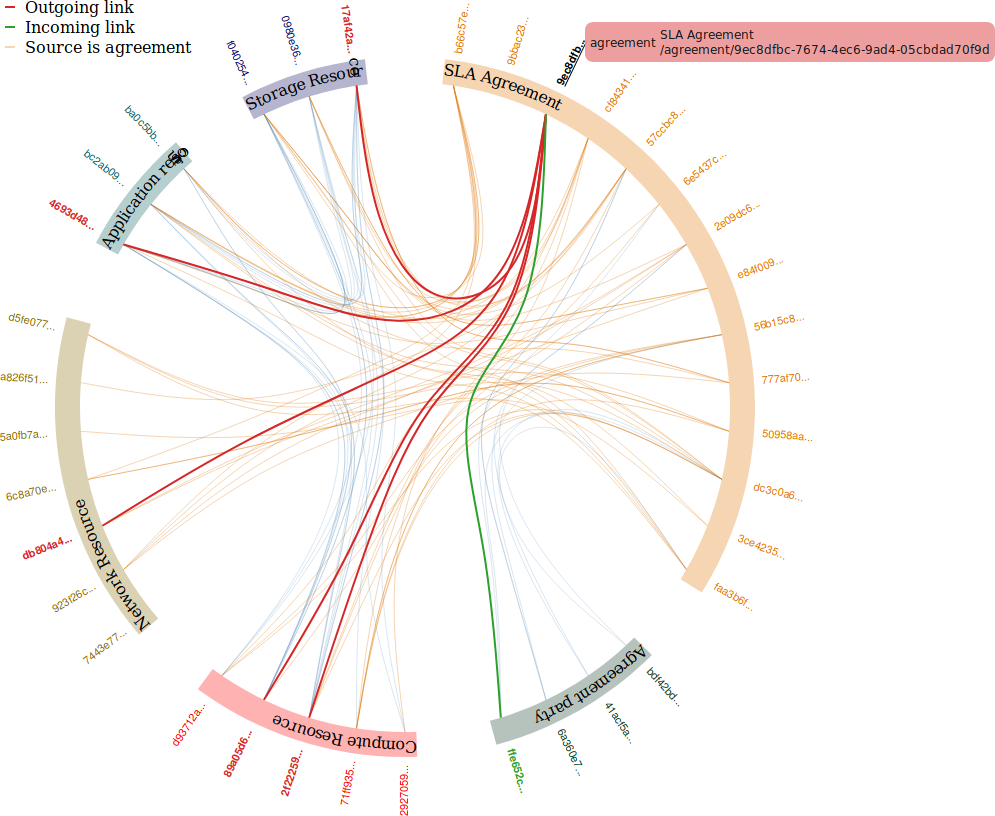
\includegraphics[width=\textwidth]{images/OCCI-relations.png}
		\caption{OCCI verknüpft Dienstgüte-Vereinbarungen mit verteilten Anwendungen, Stakeholdern und Cloud-Ressourcen. Die Zuordnung erfolgt Service-bezogen. In der Abbildung ist eine Vereinbarung markiert: Sie wird von einem Anwender beantragt (grüne Linie) und wirkt anschließend auf Ressourcen und darauf aufbauenden Anwendungen (rote Linien). Visualisierung über OCCIViz.}
		%		https://github.com/IntelLabsEurope/OCCIViz	
		\label{fig:occi}
	\end{figure}
	
	Auch hier existiert eine experimentelle Implementierung für OpenStack\footnote{\url{https://github.com/openstack/ooi}}. Diese ist jedoch bereits als obsolet gekennzeichnet. Die SLA-Unterstützung ist über ein weitere Projekt theoretisch verfügbar\footnote{\url{https://github.com/IntelLabsEurope/OCCI-SLAs}}.
	
	TOSCA und OCCI überschneiden sich nicht: Letzteres dient nicht der Modellierung Provider-übergreifender Infrastrukturen, sondern ausschließlich der Kommunikation mit der Plattform. Beide Standards ergänzen sich außerdem mit dem \emph{Cloud Data Management Interface (CDMI\footnote{\url{https://www.snia.org/cloud}})} für Verwaltung und Zugriff auf Netzwerkspeicher. Konzeptionell wurden die Standards bereits zu einem modellbasierten Cloud-Orchestrationstool verbunden.
	%Model Driven Cloud Orchestration by Combining TOSCA and OCCI (Position Paper)
	%Fabian Korte, Johannes Martin Erbel, Jens Grabowski
	
	Um sinnvoll nutzbar zu sein, müsste der offene API-Standard von Cloud-Providern implementiert werden. Da dies nicht absehbar ist, bleibt OCCI zumindest als interessante Grundlage für die API einer eigenen Cloud-Management-Plattform. Als pragmatischer Ersatz für den Zugriff auf Public-Cloud-Angebote, muss der Einsatz einer Multi-Cloud-Bibliothek evaluiert werden, siehe \autoref{sec:bibliotheken}.		
	
\end{description}

\noindent
Container sind nicht für jede Anwendung einsetzbar. Entsprechend müssen auch klassische virtuelle Maschinen bei einer Multi-Cloud-Migration unterstützt werden. Proprietäre Lösungen sind genauso ungeeignet wie Teillösungen auf einer einzelnen Service-Ebene.

Insgesamt ist der Support für offene Standards im Open-Source-IaaS-Projekt OpenStack am größten. Auf allen Ebenen der Service-Bereitstellung sind zumindest experimentelle Implementierung verfügbar: \emph{cloud-init} zur Imagekonfiguration, \emph{TOSCA} zur Service-Definition und \emph{OCCI} zur Kommunikation mit der Cloud unter Berücksichtigung von SLAs. 

Einige weitere technische Herausforderungen löst ein Multi-Cloud-Broker oder eine CMP: Management von statischen und virtuellen IPs, SSL-Zertifikaten, sowie Load Balancing. Andere Migrationshürden bleiben: Verfügbarkeit von Betriebssystemen, Frameworks und Bibliotheken, ebenso wie die Vereinbarkeit mit vorhandenen Lizenzen. Der folgende Abschnitt gibt eine Übersicht kommerzieller Cloud Management Plattformen sowie bisheriger Forschung zu Inter- und Multi-Cloud-Brokern mit besonderem Blick auf SLAs und Policys. 

\section{Die Limitierungen Kommerzieller CMPs}

Kommerzielle Anbieter wie \emph{RightScale} betonen den Self-Service-Charakter und potentielle Kosteneinsparungen durch ihrer Cloud-Management-Lösungen: Traditionell werden virtuelle Maschinen bei Bedarf von der internen IT bereitgestellt. Dabei entstehen auf der einen Seite Wartezeiten und auf der anderen erhöhter Arbeitsaufwand. 

Eine CMP kann diese Arbeiten automatisieren. Sie helfe laut \emph{Rightscale} die \emph{Schatten-IT} abzubauen -- die entsteht, wenn Mitarbeiter aufgrund langwieriger interner Prozesse zu Public-Cloud-Angeboten greifen -- mit allen negativen Folgen für Sicherheit und Vertraulichkeit. Die automatische Durchsetzung von Policys könnte sich also doppelt lohnen. Nebenbei liefert die CMP einen Preis- und Feature-Überblick der internen und öffentlichen Angebote. So hilft sie das optimale Angebot zu finden.

Nichtsdestotrotz sollte die CMP unabhängig entwickelt und betrieben werden. Cloud-Provider-eigene Lösungen werden daher nicht betrachtet. Weniger geeignet sind auch SaaS-Angebote: Hier entsteht eine neue Abhängigkeit und \emph{Single Point of Failure}. Der nachfolgende Aufzählung zeigt die aktuell verbreitetsten CMP-Lösungen mit besonderem Fokus auf Bereitstellungsmodelle, Funktionsumfang und Offenheit der Schnittstellen.

\todo{(Zusatz) Tabelle}

%Automatisierung oder nur schöne Dashboards?

\begin{description}
	
	\item[Red Hat CloudForms\footnotemark]\footnotetext{\url{https://www.redhat.com/en/technologies/management/cloudforms/}}
	Kommerzielle Cloud Management Platform, Grundlage ist das Open Source-Projekt  ManageIQ\footnotemark\footnotetext{\url{https://manageiq.org/}}, das alle wichtigen IaaS-Provider unterstützt (AWS, Azure, GCP, OpenStack).	
	
	Besonderheit: ein umfangreiches -- optional grafisches -- Policy-Management. Eigene Regeln folgen dem Schema \emph{Bedingung/Ereignis-Aktion}.
	
	Alle Schnittstellen der CMP sind proprietär. Die Orchestrierung liest jedoch vorhandene Vorlagen aus \emph{AWS CloudFormation} and \emph{OpenStack Heat}.
	%http://manageiq.org/docs/reference/latest/doc-Policies_and_Profiles_Guide/miq/
	
	\item[Rightscale CMP\footnotemark]\footnotetext{\url{https://www.rightscale.com/}}
	Proprietäres \emph{Software-as-a-Service}-Angebot, unterstützt alle wichtigen IaaS-Provider, zusätzlich Plattformdienste, Docker-Container und Hypervisoren, besonders \emph{VMware vSphere}.
	
	Infrastruktur und Dienste werden als Vorlagen in einem eigenen Katalog bereitgestellt. Dabei erlaubt Rightscale auch heterogene Anwendungen über IaaS-, CaaS- und PaaS-Grenzen hinweg.
	
	Ein Dashboard zeigt Empfehlungen zur Kostenoptimierung, allerdings ohne SLAs einzubeziehen.
	
	\item[Scalr] 
	
	%	Whitepaper! 
	
	\item[Cloudify\footnotemark]\footnotetext{\url{https://cloudify.co/}} implementiert den TOSCA-Standard und ist in einer Open-Source-Version erhältlich. Mithilfe (grafischer) Werkzeuge lassen sich Cloud-Infrastrukturen und Services modellieren. Plugins erweitern Cloudify um wichtige Provider; sowohl auf IaaS- (AWS, Azure, GCP, OpenStack) als auch auf CaaS-Ebene (Kubernetes). Konfiguration wie das Start-Skript kann direkt übergeben, oder über ein Tool wie Puppet weitergeleitet werden. 
	
	Einfache Policys sind integriert, mithilfe eines rudimentären Monitorings und der Provider-Plugins werden diese umgesetzt. Der (grafische) TOSCA-Editor und echtes Cluster-Management sind allerdings nur in der proprietären Enterprise-Ausgabe enthalten.


\end{description}

% https://www.embotics.com/solutions-cloud-governance
% Nur Azure und Amazon. Cloud Governance: Die richtigen Meta-Tags zu Instanzen hinzufügen. Kostenoptimierungsvorschläge, aber nur die Wahl zwischen zwei Providern.




%DivvyCloud (Commercial) 
%
%Automation Bots to schedule downtime, terminate, or re-size instances and resources so you only pay for what you use 
%
%https://divvycloud.com/product/botfactory/for-cost/ 

%
%Commercial Tools 
%
%https://www.cloudyn.com/ 
%
%close-source 
%
%only cost monitoring and optimization 
%
%Also, Rightscale, Cloudhealth, CloudCheckr 


%Apache Scalr (complex, freemium) 

\section{Bisherige Forschungsarbeiten}

Besonders interessant sind bisherige Arbeiten, die neben einer Föderation auch Hybrid- oder Multi-Cloud-Brokering unterstützen. Es sollten also keine Cloud-internen Plugins oder Agenten nötig sein.

Die folgende Übersicht geht besonders auf den Umfang der Policy- und SLA-Fähigkeiten ein: Diese sollten nicht nur während des Brokerings beachtet werden, sondern kontinuierlich zur Laufzeit. Auch die Einhaltung von Standards zu Service- und Ziel-Definitionen, sowie Kommunikation sind relevant. Unterschiede gibt es bei der Art unterstützter Anwendungen; neben Stapelverarbeitungsjobs und High-Performance-Computing sollten auch reguläre, interaktive Web-Anwendungen verwaltet werden können. 

Auch nicht-funktionale Anforderungen werden betrachtet: Sind die Artefakte der Projekte noch als Code verfügbar oder sogar in Open-Source-Tools und kommerziellen Produkten aufgegangen?

%policy-driven service placement optimization in federated clouds 


\begin{description}	
	
	
	\item[InterCloud] ist ursprünglich eine Föderation von Cloud-Ressourcen. Auf einem zentralen Marktplatz \emph{zeigen} Clouds ihre Dienste, oder \emph{kaufen} sie je nach Bedarf. Für diese aktive Teilnahme sind Cloud-interne Agenten nötig.
	
	Vorgeschlagen werden zusätzlich externe Adapter, über die einerseits Provider \emph{unfreiwillig} in die Föderation integriert werden, andererseits aber auch weitere Teilnehmer Ressourcen kaufen können. Hierüber könnten auch Anwendungsbroker die Ressourcen der Föderation nutzen.
	
	Der Ansatz fokussiert sich stark auf das Preis-gesteuerte Brokering, beachtet optional aber auch Geostandorte. Die Provider unterstützen eingeschränkt SLAs. Verteilt werden nur Rechenaufgaben, interaktive Anwendungen sind nicht vorgesehen.
	%	5, 37, 38 Grozev
	
	
	\item[Contrail] ist eine zentral gemanagte Föderation. SLAs gelten für den gesamten Cloudverband, nicht für einzelne Anwendungen. Das zentrale Element, der \emph{Federation Runtime Manager}, verteilt jedoch individuelle Nutzeranfragen und beachtet dabei Preis und Leistung.
	
%	http://contrail-project.eu/architecture

	Contrail versteht sich als PaaS und unterstützt auch Hadoop. Ähnlich zu InterCloud sprechen externe Adapter theoretisch weitere Provider an, die sich der Föderation nicht bewusst sind.
		
	
	\item[RESERVOIR] entwickelt eine Peer-to-Peer-Föderation mit eigenen Service-Schemata und Inter-Cloud-Protokollen. Ein Unterprojekt abstrahiert die Cloud-Ressourcen durch eine zusätzliche Schicht, sodass Java-Anwendungen transparent auf allen Providern ausgeführt und migriert werden können. Ein Broker beobachtet Performance-SLAs und skaliert die Instanzen entsprechend.
%	IBM, Telefonica, SAP + Universites, EU-funded
	
	
	\item[Optimis] baut auf eine zentrale \emph{Deployment Engine (DE)}. Über interne und externe Adapter verbinden sich Cloud-Provider und senden ihre Ressourcen-Angebote. Soll eine Anwendung ausgerollt werden, wählt die DE passende Provider aus und sendet ihnen ein SLA-Template. Diese antworten mit einer Zusage, Absage oder einem Gegenvorschlag. Aus allen Antworten wählt der DE anschließend das beste Angebot. Dabei beachtet sie quantitative Größen wie den Preis, aber auch Erfahrungswerte wie Zuverlässigkeit oder die Energieeffizienz eines Providers.
	
	Die internen Adapter vertreten Föderationsmitglieder -- sie lehnen eine Anfrage des DE ab, wenn sie für den Cloud-Provider finanziell unattraktiv ist. Eine weitere Komponente, der \emph{Service Optimizer}, beobachtet alle Anwendungen auf SLA-Verletzungen. Wie genau SLAs spezifiziert werden können ist nicht deutlich. Auch der Matching-Algorithmus ist nicht öffentlich. Geostandorte werden nicht beachtet. Externe Adapter sind rein konzeptionell und nicht implementiert.
	
	Die Arbeit geht auch auf die Bereitstellung von Laufzeitumgebungen und Provider-spezifischen Images ein: Er schlägt eine Erweiterung des \emph{Open Virtualization Formats (OVF)} vor. Zusätzliche Metadaten beschreiben die nötige Cloud-Konfiguration.
	
	
	\item[Bernsetein InterCloud Blueprint] Eine weltweite Föderation der Cloud-Ressourcen. Interessant ist der dezentrale Ansatz des Brokerings. Nur in dieser Arbeit wird der Broker als \emph{Single Point of Failure} erkannt: deshalb soll er zwangsläufig repliziert und in allen Regionen mindestens einmal verfügbar sein. Der Ansatz folgt also den Grundlagen des Internets und entwickelt eigene Inter-CLoud-Protokolle auf Basis von XMPP und RDF.
	
	
	\item[STRATOS] ist eine Cloud-Management-Plattform mit integriertem Multi-Cloud-Broker. Anwendungen werden über das eigenentwickelte, XML-basierte \emph{Topology Descriptor File (TDF)} beschrieben. Es enthält die Service-Architektur und zusätzlich Policys und SLOs. Für den Zugriff auf externe Clouds existiert ein \emph{Translation Layer}, der eine einheitliche API bereitstellt. Die Arbeit fokussiert sich auf die Bereitstellung klassischer Web-Anwendungen und Kostenoptimierung. Der mittlerweile nicht mehr weiterentwickelte \emph{Service Measurement Index (SMI)} definiert die Ziele.
%	https://www.google.de/url?sa=t&rct=j&q=&esrc=s&source=web&cd=1&ved=0ahUKEwju27vHs6DZAhUCWRQKHRv7BEcQFggrMAA&url=http%3A%2F%2Fwww.mikesmit.com%2Fwp-content%2Fpapercite-data%2Fpdf%2Fcloud2012.pdf&usg=AOvVaw3e6yhHYmhWBbIxtr7MqkuX
	
	\item[Meryn] ist eines der wenigen Implementierung eines SLA-bezogenen PaaS-Systems. Aktuelle Plattformen begrenzen hauptsächlich den Ressourcenverbrauch der Gastanwendungen -- Meryn schlägt zusätzlich eine Kostenoptimierung für Provider vor.
	
	Cloud-interne \emph{Cluster-Manager} bieten in einem Wettbewerb um Ausführungsaufträge. Die Arbeit fokussiert sich auf Stapelverarbeitung mit Hadoop und anderen Framworks. Dabei entwickeln die Autoren für jedes Framework eine eigene VM, die jeweils einmal pro Cluster ausgeführt wird. Vorgestellt wird außerdem ein \emph{Cloud-Bursting-Ansatz}, bei dem zusätzliche Ressourcen in Public Clouds angemietet werden.
	
	
	\item[SeaClouds] ist ein EU-finanziertes PaaS-Management-Projekt mit großem Umfang. Vorgeschlagen wir ein Referenzmodell aus \emph{Planner}, \emph{Deployer}, \emph{SLA Service} und \emph{Monitor}. Hierüber lassen sich verteilte Anwendungen modellieren, auf verschiedenen Providern bereitstellen und SLA-bezogen verwalten.
	
	Besonderheit ist die Unterstützung von offenen Standards wie der \emph{Cloud Application Management for Platforms} für APIs und TOSCA zur Service-Modellierung. Angebote der Cloud-Provider werden kontinuierlich überwacht und als TOSCA-Graph abgebildet. SLAs nutzen allerdings nicht TOSCA, sondern \emph{WS-Agreements}.
%	http://wsag4j.sourceforge.net/site/wsag/wsag-language.html
		
	Erwähnt wird eine Provider-unabhängige Lösung, konkret umgesetzt ist dies jedoch nur für die Open-Source-PaaS-Projekte \emph{OpenShift} und \emph{CloudFoundry}.
	
	
%	\item[An SLA-based Broker for Cloud Infrastructures] Nicht nur Private Clouds sondern auch Personal Devices 
%	
%	Modulare Architektur 
%	
%	wechselnde und unzuverlässige Provider
%	
%	Fokus auf Föderation. Aber: Idee der forced integration of commercial cloud providers 
	
\end{description}


%Mist.io Open source 
%Build on libcloud and cloudify
%Can monitor costs (commercial)
%No automatic scheduling 

\noindent
Im Gegensatz zu den kommerziellen Projekten liegt der Fokus vieler Forschungsarbeiten auf Cloud-Föderationen und SLA-basiertem Brokering. Einige unterstützen über Adapter konzeptionell mehrere Bereitstellungsmodelle; je nachdem, ob dem Cloud-Provider die Mitgliedschaft in einer Föderation bewusst ist. Interne Adapter sprechen mit zusätzlichen, Cloud-internen Erweiterungen. Externe Adapter nutzen die öffentlichen APIs von Drittanbieter-Clouds. Hier entsteht zwar Mehraufwand, dieser könnte in weiteren Entwicklungen jedoch von einer Multi-Cloud-Bibliothek abgemildert werden.

Negativ fällt auf, dass die Artefakte der meisten (EU-)Forschungsprojekte
nicht mehr verfügbar sind. Auch Matching-Algorithmen sind teilweise nicht veröffentlicht. Die Ergebnisse lassen sich so nicht mehr nachvollziehen. Ohnehin basieren sie oft auf veralteten Technologien: Formate wie OVF werden in modernen IaaS-Plattformen nicht mehr unterstützt. Demgegenüber spielen Container oder Serverless-Computing keine Rolle.

Wie bereits beschrieben, existieren eine Vielzahl von offenen Cloud-Standards. Von Service-Definition über SLAs bis zur standardisierten Kommunikation mit der Management Plattform. In der Forschung werden diese aber nur selten aufgegriffen und stattdessen neu erfunden. Besonders deutlich wird die in einer Forschungsübersicht der Europäischen Kommission.
%Cloud Computing Service Level
%Agreements
%Exploitation of Research Results
%Editor: Dimosthenis Kyriazis
Das eigentliche Problem der Portabilität im Cloud-Umfeld lässt sich so nicht lösen.

Insgesamt bleibt vor allem die unterschiedliche Ausrichtung von Forschungsprojekten und kommerziellen Anbietern: Forschungsprojekte fokussieren sich auf Föderationen. Dies entspricht auch dem vorherrschenden Cloud-Typ innerhalb der verantwortlichen Organisationen. SLAs werden ausschließlich von diesen ausgewertet und teilweise umgesetzt. Kommerzielle Projekte sind dagegen meist externe Broker, stellen Preisunterschiede und Kosten dar. Statt SLAs beachten sie nur einfache Policys.

Der folgende Abschnitt erstellt aus den bisherigen Überlegungen zu Anforderungen, Schemata und Forschungsergebnissen einen Vorschlag für SLA-basiertes Brokering auf Basis moderner Technologien.


\section{Modularer Architektur-Vorschlag}

%Komponenten des Brokers.
%
%
%In der CMP: Polling oder Notification?
%
%Was löst eine Aktion aus?
%- Monitoring der Services
%- Änderung der Umgebung
%- User-Aktion
%- Ergebnis einer anderen Policy

\begin{figure}
	\centering
	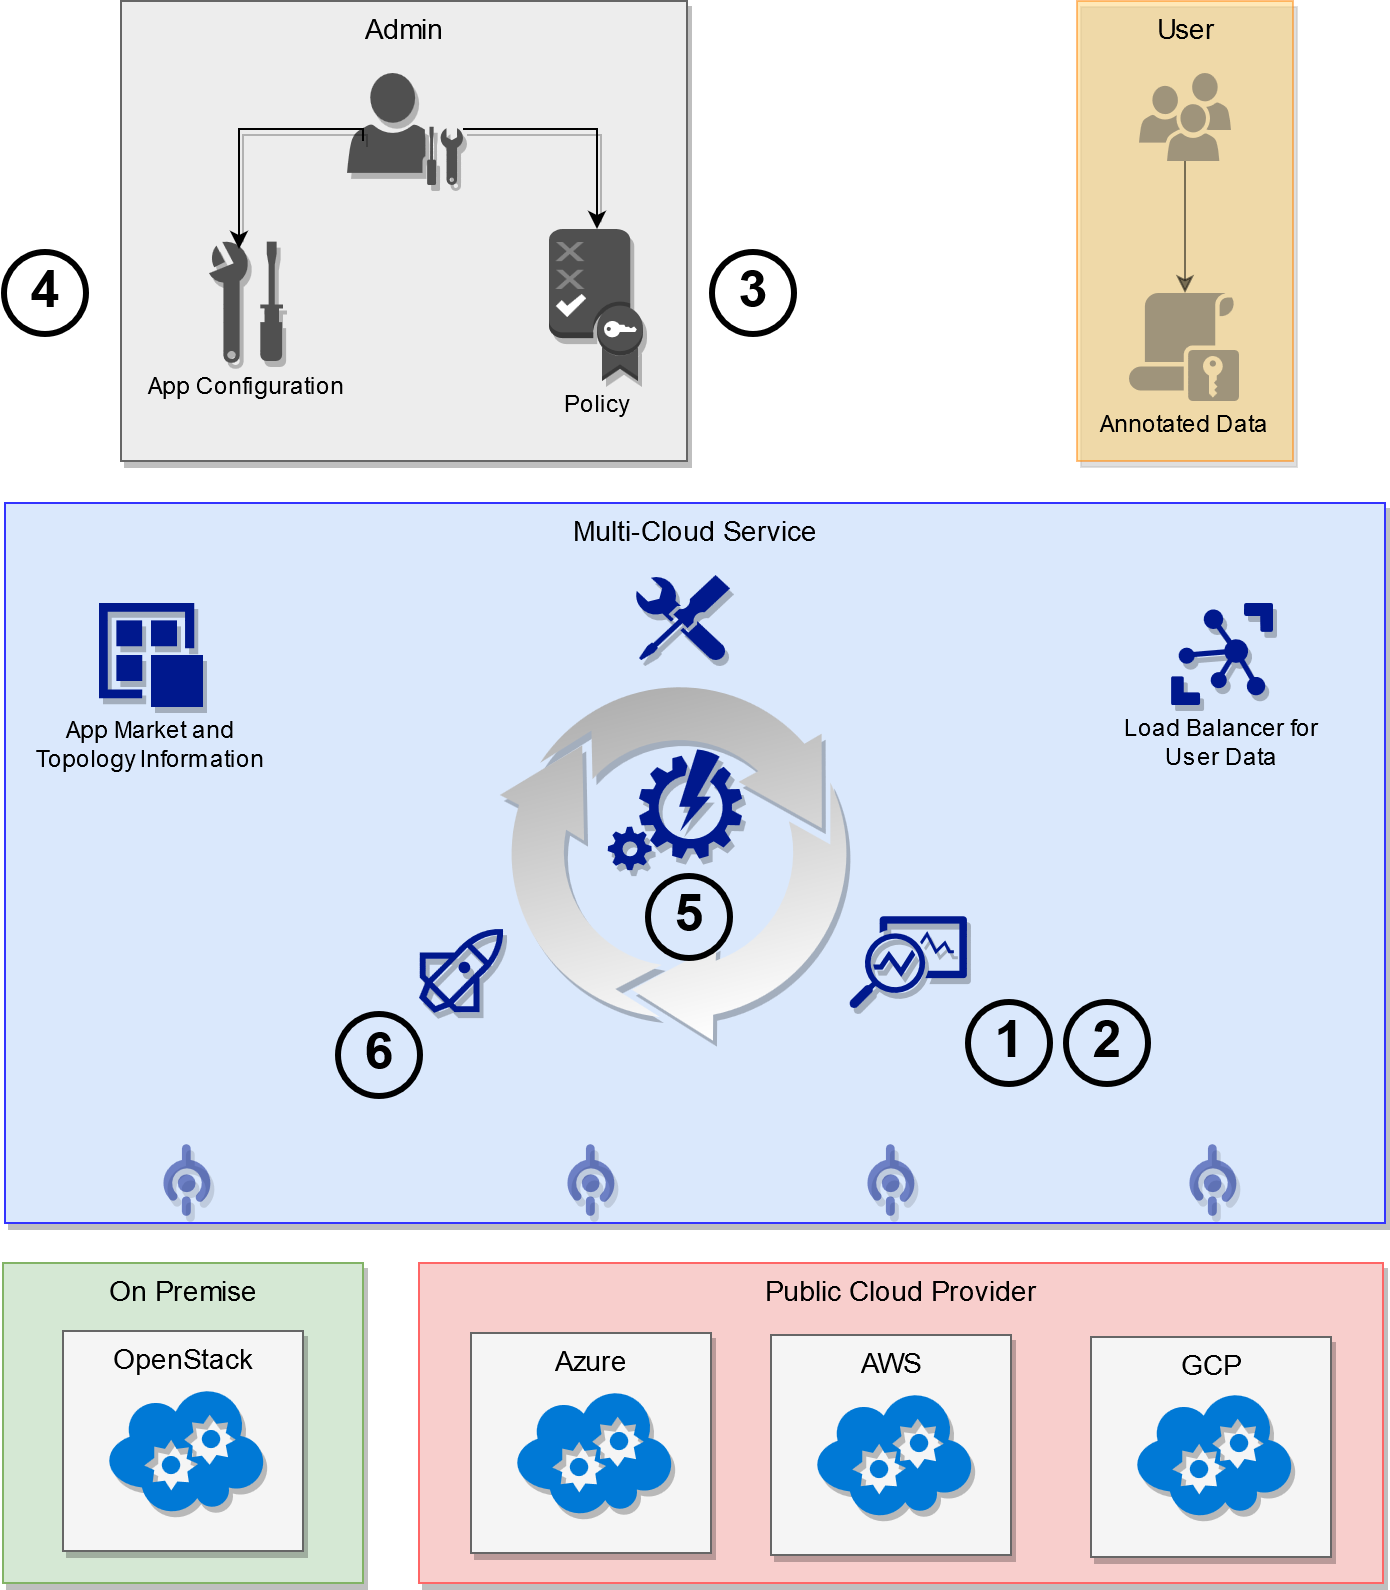
\includegraphics[width=0.9\linewidth]{images/cycle}
	\caption{}
	\label{fig:cycle}
\end{figure}

%Zyklus\autoref{fig:cycle}:

%\begin{description}
%	\item[Nummerierte Aufzählung]~\par
\begin{enumerate}
	
	\item Sammeln der Meta-Informationen alle Cloud-Provider
	\begin{enumerate}
		\item Kapazität (CPU, RAM, HDD, Network)
		\item Features (Verschlüsselung, CUDA, …)
		\item Geo-Lokation 
		\item Preis
	\end{enumerate}
	
	\item Sammeln der Laufzeitinformationen der PaaS/Anwendungen
	\begin{enumerate}
		\item Auslastung
		\item Fehler
		\item Ausfälle
	\end{enumerate}
	
	\item Sammeln der SLAs
	\begin{enumerate}
		\item Policy-Definitionen
		\item Policy-Konfiguration
		\item Placement-Algorithmen
	\end{enumerate}

	\item Neue Anwendung/Änderung eines SLA
	
	\item Optimierung
	\begin{enumerate}
		\item Feste Vorgaben (Geo, Backup)
		\item Weiche (Preis, Latenz, Verfügbarkeit)
	\end{enumerate}

	
	\item Ausführung
	\begin{enumerate}
		\item Netzwerkkonfiguration
		\item Allokation/De-Allokation von Ressourcen
		\item Deployment
		\item Migration
		\item Logging/Benachrichtigung
		\item Backup
	\end{enumerate}

\end{enumerate}

\section{Brokering}
%entailing multiple constraint satisfaction (MCS)
%
%\todo{Schaubild, was wird wann gematcht}
%% Pseudocode des Algorithmus, wie in Meryn
%
%Kostenoptimierung
%
%Preisentwicklung? 
%
%Migration je nach Tageszeit? 
%
%Kosten der Datentransfers 
%
%Subscription On-Demand/Monthly/Yearly 
%
%Kompliziert durch undurchsichtige Staffelpreise
% https://www.rightscale.com/blog/cloud-cost-analysis/aws-vs-azure-vs-google-cloud-pricing-compute-instances

%https://www.rightscale.com/blog/cloud-cost-analysis/comparing-cloud-instance-pricing-aws-vs-azure-vs-google-vs-ibm

%
%Cost Calculators 
%
%http://go.appscale.com/cloud-cost-calculator-help 
%
%https://github.com/ifosch/accloudtant 
%
%https://awstcocalculator.com/# 
%